%% Copyright 1998 Pepe Kubon
%%
%% `two.tex' --- 2nd chapter for thes-full.tex, thes-short-tex from
%%               the `csthesis' bundle
%%
%% You are allowed to distribute this file together with all files
%% mentioned in READ.ME.
%%
%% You are not allowed to modify its contents.
%%

%%%%%%%%%%%%%%%%%%%%%%%%%%%%%%%%%%%%%%%%%%%%%%%%%
%
%     Chapter 4  
%
%%%%%%%%%%%%%%%%%%%%%%%%%%%%%%%%%%%%%%%%%%%%%%%%

\chapter{A Pruning-based Method on Graphs}
\label{ch:graph}

In this chapter, we will introduce the algorithms to compute the skyline subspace queries. One way to solve this problem is to compute the label distance vectors of all the vertices first and enumerate all subspaces to check whether the query vertex is a subspace skyline in those subspaces using the existing skyline computation algorithms. Given a label graph $G=(V, E, L)$, the time complexity of this method is $O((|V|+|E|)|L| + 2^{|L|}|L|^2)$ which is very time consuming. In order to make the algorithm more efficient, we propose a bottom-up set enumeration algorithm and manage to avoid some unnecessary computation by applying some pruning techniques in our method.

\begin{table}[h]
\centering
\begin{tabular}{|l|p{11cm}|}
\hline
Symbol                      & Interpretation                                                                                                                                     \\ \hline
$q$                         & query vertex $q$                                                                                                                                   \\ \hline
$LV_v$                      & label distance vector of vertex $v$ representing the distances between $v$ and each label.                                                         \\ \hline
$\mathcal{B}$               & subspace $\mathcal{B}$                                                                                                                             \\ \hline
$\mathit{SDS}_u$            & strictly dominating subspace of $u$                                                                                                                \\ \hline
$\mathit{EQ}_u$             & equivalence subspace of $u$                                                                                                                        \\ \hline
$\mathit{CAND}_\mathcal{B}$ & dominating candidate set of subspace $\mathcal{B}$                                                                                                 \\ \hline
$(u, dom)$                  & element in dominating candidate set. $(u, dom) \in \mathit{CAND}_\mathcal{B}$ means that $u$ dominates query vertex $q$ in subspace $\mathcal{B}$. \\ \hline
$(u, eq)$                   & element in dominating candidate set. $(u, eq) \in \mathit{CAND}_\mathcal{B}$ means that $u$ dominates query vertex $q$ in subspace $\mathcal{B}$.  \\ \hline
\end{tabular}
    \caption{Symbols Used in the Pruning-based Method on Graph}
    \label{tab:symbol_graph}
\end{table}

\section{BFS Label Collecting}
\label{sec:bfs-collect}
We collect the $d$-hop labels using Breadth-First-Search and get the \emph{label distance vector} of query vertex. The idea is that we start with our query vertex and traverse the graph in the Breadth First order. If we visit a vertex with a new label that we have not visited before, we update the corresponding entry of that label in the \emph{label distance vector} to the distance from the query vertex. The Breadth First Search process will end if all reachable vertices in $d$ hops has been visited. And we will get the \emph{label distance vector} of the query vertex when the BFS label collecting ends.

\begin{algorithm}[H]
  \caption{Label Collecting}
  \label{algo:graph_collect}
  \begin{algorithmic}[1]
  \show\LOOP
    \REQUIRE A graph $G=(V,E)$, a list of label sets $F=\left\{L_v | v \in V\right\}$, the label sets of all vertices, a query vertex $q$, the number of hops $d$;
    \ENSURE The label distance vector $LV_q$ of the query vertex $q$;
    \STATE push $\left(q, 0\right)$ to $Q$
    \WHILE {$Q$ is not empty}
        \STATE $\left( v, dis\right)$ = de-queue $Q$
        \IF{$dis=d$}
            \STATE continue
        \ENDIF
        \FORALL {not visited neighbour $u$ of $v$}
            \STATE push $\left(u, dis+1\right)$ to $Q$
            \FORALL {label $l$ in $L_u$}
                \IF {($l$, $\ast$) not in $LV_q$}
                    \STATE add ($l$, $dis+1$) to $LV_q$
                \ENDIF
            \ENDFOR
        \ENDFOR
    \ENDWHILE
  \end{algorithmic}
\end{algorithm}

\section{Dominating Candidate Sets}
\label{sec:dom-cand}

By collecting the label in $d$ hops from the query vertex, we build the label distance vector of our query vertex. To avoid computing the label distance vectors of some unnecessary vertices, we define a concept of dominating candidate set to store the possible vertices that dominate the query vertex $q$ in certain subspaces. Given a subspace $\mathcal{B}$, Dominating Candidate Set of $\mathcal{B}$ contains the vertices that may dominate the query vertex on some subspace $\mathcal{C}$ such that $\mathcal{B} \subset \mathcal{C}$.

\begin{definition}[Dominating Candidate Set]
Given a subspace $\mathcal{B}$, the dominating candidate set of that subspace is the set of vertices that dominate the query vertex $q$ or equal to query vertex $q$ in subspace $\mathcal{B}$, denoted by $\mathit{CAND}_\mathcal{B}$.
\end{definition}

The reason we put all vertices equal to the query vertex to the candidate set is that if a vertex equals to the query vertex in a subspace $\mathcal{B}$ then that vertex may dominate the query vertex in some supersets of subspace $\mathcal{B}$. 

If $\mathit{CAND}_\mathcal{B} = \emptyset$ or every vertex in $\mathit{CAND}_\mathcal{B}$ is equal to the query vertex $q$ in subspace $\mathcal{B}$, then $q$ is a skyline in subspace $\mathcal{B}$. Therefore, we can determine whether a subspace $\mathcal{B}$ is a \emph{skyline subspace} by checking whether the dominating candidate set of $\mathcal{B}$ or whether all elements in \emph{dominating candidate set} of $\mathcal{B}$ are equal to the query vertex in subspace $B$. To understand the concept of dominating candidate set, we will show a running example in Section~\ref{dom:run_ex}.

\subsection{Dominating Candidate Set of $1$-dimensional subspace}

We will introduce an algorithm to compute the \emph{dominating candidate set} of $1$-dimensional subspace. We will also introduce the concepts of \emph{Strictly Dominating Subspace} and \emph{Equivalence Subspace} which help us prune the unnecessary dominating candidate.

\begin{definition}[Strictly Dominate]
In a label graph, we say that label distance vector $LV_v=\left\{(l_i, dist_i)\right\}$ strictly dominates label vector $LV_u=\left\{(l_i, dist_i^\prime)\right\}$, if and only if for all i, $dist_i < dist_i^\prime$.
\end{definition}

\begin{definition}[Strictly Dominating Subspace]
Given a vertex $u$, strictly dominating subspace $\mathcal{B}$ for $u$ is the maximal subspace such that $u_\mathcal{B}$ strictly dominates query vertex $q_\mathcal{B}$ on subspace $\mathcal{B}$, denoted as $\mathit{SDS}_u$.
\end{definition}

\begin{definition}[Equivalence Subspace]
Equivalence subspace $\mathcal{B}$ is the maximal subspace such that given a vertex $u$, $u_\mathcal{B}$ equals to the query vertex $q_\mathcal{B}$ in subspace $\mathcal{B}$, denoted by $\mathit{EQ}_u$.
\end{definition}

In this algorithm, we start from the vertices with labels and update the label distance vectors of those vertices. In the next step, we push all the neighbours of those vertices into a queue and update their label distance vectors and keep going. 
\begin{algorithm}[h]
  \caption{Dominating candidate Set on $1$-Dimensional Subspace}
  \label{algo:dom_cand_graph}
  \begin{algorithmic}[1]
  \show\LOOP
    \REQUIRE A graph $G=(V,E)$ and the label vector $LV_q$ of the query vertex $q$;
    \ENSURE Dominating candidate Set $\mathit{CAND}$ in all one dimension subspace in $LV_q$, $\mathit{EQS}$ and $\mathit{SDS}$;
    \FORALL {vertex $v$ contains label $l$}
        \FORALL {$\left(l, dist\right)$ in $LV_q$}
            \STATE push $\left(v, 0\right)$ to $Q$
        \ENDFOR
    \ENDFOR
    \WHILE {$Q \not= \emptyset$}
        \FORALL {$\left(l, dist\right)$ in $LV_q$}
            \STATE $\left(v, dist_{v,l}\right)$ = de-queue $Q$
            
            \IF{$dist_{v,l} = dist$}
                \STATE add $\left(u, equal\right)$ to $\mathit{CAND}_l$
                \STATE add $l$ to $\mathit{EQS}_u$
                \STATE continue
            \ENDIF
            \STATE add $\left(u, dom\right)$ to $\mathit{CAND}_l$
            \STATE add $l$ to $\mathit{SDS}_u$
            \FORALL {not visited neighbour $u$ of $v$}
                \STATE push $\left(u, dist_{v,l}+1\right)$ to $Q$
            \ENDFOR
        \ENDFOR
    \ENDWHILE
  \end{algorithmic}
\end{algorithm}

\subsection{Running Example of Computing Dominating candidate Set}
\label{dom:run_ex}
In this subsection, we will give an example of how the algorithm of finding \emph{dominating candidate set on $1$-dimensional subspace} works. We will also show how the \emph{strictly dominating subspace} and the \emph{equivalence subspace} of each vertex are built.

\begin{figure}[H]
    \centering
    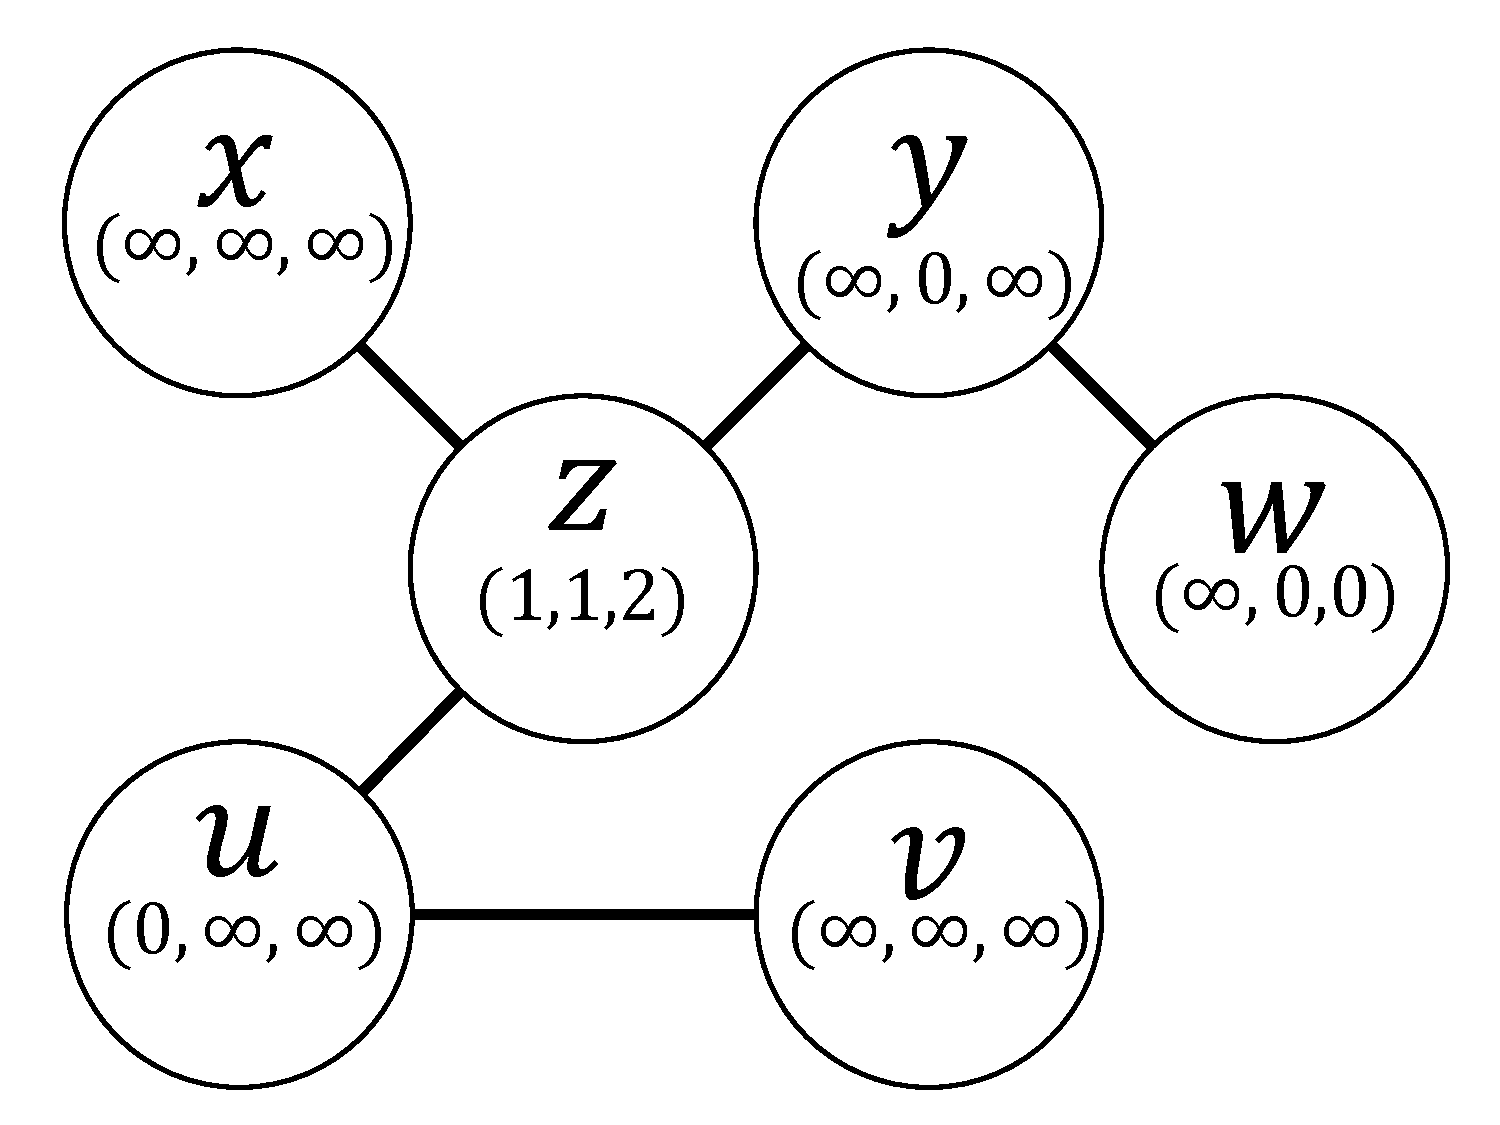
\includegraphics[width=0.5\textwidth]{figs/graph_example_1}
    \caption{Label distance vector on the first iteration}
    \label{fig:cand_step1}
    
\end{figure}

\begin{table}[H]
    \centering
    \begin{tabular}{|l|l|l|}
    \hline
      & SDS         & EQS         \\ \hline
    u & A           & $\emptyset$ \\ \hline
    v & $\emptyset$ & $\emptyset$ \\ \hline
    w & BC          & $\emptyset$ \\ \hline
    x & $\emptyset$ & $\emptyset$ \\ \hline
    y & B           & $\emptyset$ \\ \hline
    \end{tabular}
    \caption{SDS and EQS of each vertex on the first iteration}
    \label{tab:sds_step1}
\end{table}

\begin{table}[H]
    \centering
    \begin{tabular}{|l|l|}
    \hline
    Subspaces & Dominating candidate \\ \hline
    A         & $(u, dom)$            \\ \hline
    B         & $(w, dom), (y, dom)$            \\ \hline
    C         & $(w, dom)$            \\ \hline
    \end{tabular}
    \caption{Dominating candidate set of each $1$-dimensional subspace on the first iteration}
    \label{tab:cand_set_step1}
\end{table}

Consider the LinkedIn network represented by Table~\ref{tab:skill_sets} and Figure~\ref{fig:graph} as our running example. Again, we take $z$ as the query vertex. The label distance vectors of all vertices are originally initialized as ($\infty$, \dots, $\infty$). As shown in Figure~\ref{fig:cand_step1}, we start from the vertices with labels and mark the corresponding entries of the label distance vectors of those vertices as $0$. 
We add the label $A$ to $\mathit{SDS}_u$ because $u$ dominates the query vertex $z$ in dimension $A$. Table~\ref{tab:sds_step1} shows the $\mathit{SDS}$ and $\mathit{EQS}$ of all the vertices in the first iteration.
In the first iteration, since $u$ dominates $z$ in the $1$-dimensional subspace $A$, we add $(u, dom)$ to the dominating candidate set $\mathit{CAND}_A$ as shown in Table~\ref{tab:cand_set_step1}.

\begin{figure}[H]
    \centering
    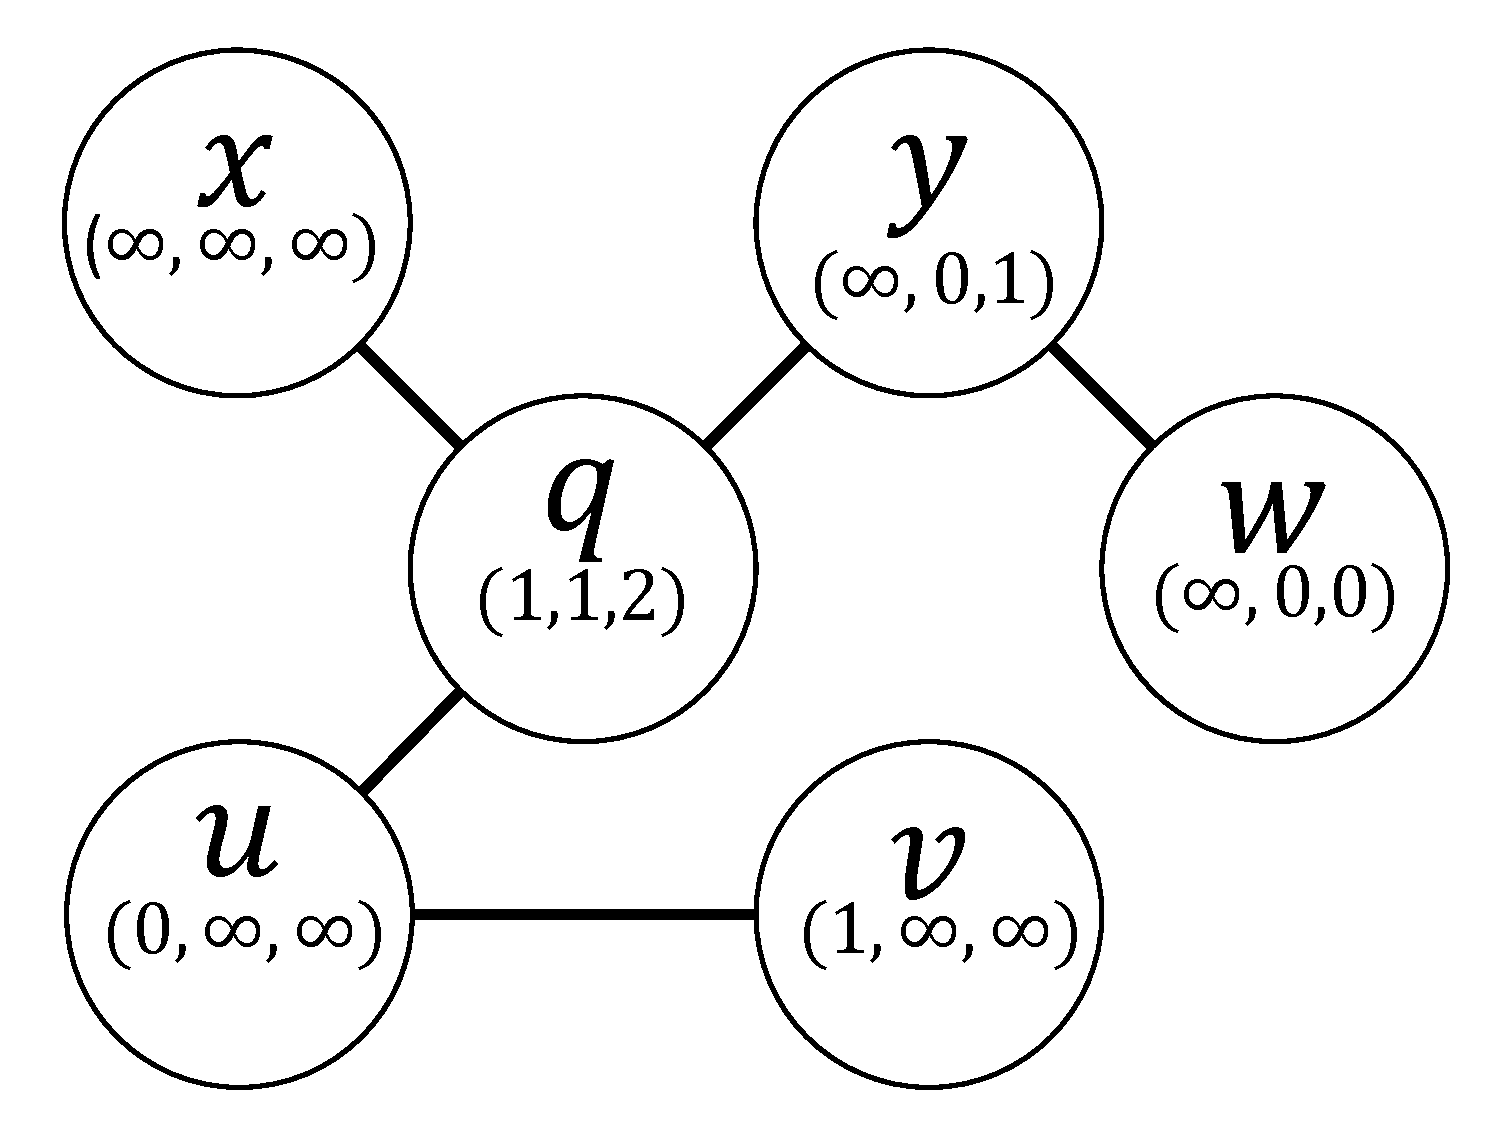
\includegraphics[width=0.5\textwidth]{figs/graph_example_2}
    \caption{Label distance vector on second iteration}
    \label{fig:cand_step2}
\end{figure}

\begin{table}[H]
    \centering
    \begin{tabular}{|l|l|l|}
    \hline
      & SDS         & EQS         \\ \hline
    u & A           & $\emptyset$ \\ \hline
    v & $\emptyset$ & A           \\ \hline
    w & BC          & $\emptyset$ \\ \hline
    x & $\emptyset$ & $\emptyset$ \\ \hline
    y & BC          & $\emptyset$ \\ \hline
    \end{tabular}
    \caption{SDS and EQS of each vertex on the second iteration}
    \label{tab:sds_step2}
\end{table}

\begin{table}[H]
    \centering

    \begin{tabular}{|l|l|}
    \hline
    Subspaces & Dominating candidate \\ \hline
    A         & $(u, dom), (v, eq)$            \\ \hline
    B         & $(w, dom), (y, dom)$            \\ \hline
    C         & $(w, dom), (y, dom)$            \\ \hline
    \end{tabular}
    \caption{Dominating candidate set of each $1$-dimensional subspace on the second iteration}
    \label{tab:cand_set_step2}
\end{table}


Then, we explore the graph in a breadth first manner. On the second iteration, as shown in Figure~\ref{fig:cand_step2}, we visit the neighbours of the vertices that have been visited in the first iteration and update the corresponding entries of their label distance vectors. Table~\ref{tab:sds_step2} shows that subspace $A$ is added to $\mathit{EQS}_v$ because on the second iteration we update the distance between $v$ and label $A$ to $2$ which is equal to the distance between $z$ and label $A$. For the same reason, we add $(v, eq)$ to $\mathit{CAND}_A$ as shown in Table~\ref{tab:cand_set_step2}. It means that in $1$-dimensional subspace $A$, $v$ is equal to $z$ and it is still possible for $v$ to dominates $z$.

After two iterations, the process of building the dominating candidate sets of all $1$-dimensional subspace ends. \emph{Strictly dominating subspace} and \emph{equivalence subspace} of all the vertices on graph are built. In Figure~\ref{tab:d_hops_distance}, we collect the $3$-hop labels by Breadth-First-Search and get the label vectors. By this point, if the value of label $l$ in label distance vector of vertex $v$ is $\infty$, then it means the distance between label $l$ and vertex $v$ is longer than the distance between the label $l$ and the query vertex $q$.

\begin{table}[h]
    \centering
    \begin{tabular}{llll}
    \hline
    Distances & A & B & C \\ \hline
    $u$       & 0 & $\infty$ & $\infty$ \\ \hline
    $v$       & 1 & $\infty$ & $\infty$ \\ \hline
    $w$       & $\infty$ & 0 & 0 \\ \hline
    $x$       & $\infty$ & $\infty$ & $\infty$ \\ \hline
    $y$       & $\infty$ & 0 & 1 \\ \hline
    $z$       & 1 & 1 & 2 \\ \hline
    \end{tabular}
    \caption{Distances between each person and each skill in 2-hop}
    \label{tab:d_hops_distance}
\end{table}

Although some information is still missing (equal to $\infty$) in Table~\ref{tab:d_hops_distance}, we are still able to get the mininmal skyline subspaces of $z$: $(A, B)$ and $(A, C)$ from the Table~\ref{tab:d_hops_distance}.

\section{Dominating candidate Pruning}

In this section, we will introduce a way to prune the unnecessary vertices using the \emph{strictly dominating subspace} $SDS$ and the \emph{equivalence subspace} of the vertices.

\begin{property}
\label{ppt:prune_cand}
Pruning a vertex $u$ from $\mathit{CAND}$ if $\exists v, (SDS_u \cup EQS_u \subseteq SDS_v \cup EQS_v) \wedge (SDS_u \subseteq SDS_v)$, does not affect the result.
\end{property}

\begin{proof}
Let $u$ be a vertex that $\exists v, (SDS_u \cup EQS_u \subseteq SDS_v \cup EQS_v) \wedge (SDS_u \subseteq SDS_v)$. For the query vertex $q$ in any subspace $\mathcal{B}$, there are three different cases.\\
Case 1: $q$ is a skyline in subspace $\mathcal{B}$. Then $\mathit{CAND}_\mathcal{B}$ does not contain any elements. Pruning $u$ from $\mathit{CAND}$ does not change the result.\\
Case 2: $q$ is not a skyline in subspace $\mathcal{B}$ and $q$ is dominated by a vertex $w$, removing $u$ does not change the result.\\
Case 3: $q$ is not a skyline in subspace $\mathcal{B}$ and $q$ is dominated by vertex $u$, then $(\mathcal{B} \subseteq EQS_u \cup SDS_u) \wedge (\mathcal{B} \cap SDS_u \not= \emptyset)$, and there exists such a $v$ that ($SDS_u \cup EQS_u \subseteq SDS_v \cup EQS_v) \wedge (SDS_u \subseteq SDS_v)$. And $(\mathcal{B} \subseteq EQS_v \cup SDS_v) \wedge (\mathcal{B} \cap SDS_v \not= \emptyset)$ is satisfied.\\
Therefore $v$ also dominates $q$ and removing $u$ from $CAND$ does not affect the result.
\end{proof}

One observation is that the unnecessary points are very likely to be pruned by the neighbours of the query vertex $q$. The intuition is that usually the neighbours of query vertex $q$ will have larger \emph{Strictly Dominating Set}, comparing to the vertices that are not the neighbours of query vertex because the query vertex $q$ collects the labels directly from its neighbours and the neighbours strictly dominate the query vertex in subspaces of those labels.
By Property~\ref{ppt:prune_cand} and the observation above we develop a $1$-hop pruning algorithm. In Algorithm~\ref{algo:pruning_graph}, $s$ contains all query vertex's neighbours. If both $SDS_u$ and $SDS_u \cup EQS_u$ are subsets of $SDS_v$ and $SDS_v \cup EQS_v$ ($v \in s$) respectively, then we prune $u$ from the \emph{dominating candidate sets}.

\begin{algorithm}[H]
  \caption{1-hop Pruning}
  \label{algo:pruning_graph}
  \begin{algorithmic}[1]
  \show\LOOP
    \REQUIRE Strictly Dominating Subspace $\mathit{SDS}$, Equivalence Subspace $\mathit{EQS}$, Dominating candidate $\mathit{CAND}$, query vertex $q$, graph $G=(V, E)$;
    \ENSURE Pruned Dominating candidate $\mathit{CAND}$;
    \STATE s = $\left\{v|e(v, q) \in E \wedge (\forall u, e(u, q) \in E \wedge SDS_v \not\subset SDS_u)\right\}$
    
    \FORALL {$(l, dist)$ in $LV_q$}
        \FORALL {$u$ in $\mathit{CAND}_l$}
            \FORALL {$v$ in $s$}
                \IF {$u \not= v \wedge SDS_u \cup EQS_u \subseteq SDS_v \cup EQS_v \wedge SDS_u \subseteq SDS_v$}
                    \STATE delete $u$ from $\mathit{CAND}_l$
                \ENDIF
                
            \ENDFOR
        \ENDFOR
    \ENDFOR
  \end{algorithmic}
\end{algorithm}

\begin{table}[h]
    \centering
    \begin{tabular}{|l|l|l|l|}
    \hline
    Dim & $SDS$       & $EQS$       & $SDS \cup EQS$ \\ \hline
    $u$ & A           & $\emptyset$ & A              \\ \hline
    $v$ & $\emptyset$ & A           & A              \\ \hline
    $w$ & BC          & $\emptyset$ & BC             \\ \hline
    $x$ & $\emptyset$ & $\emptyset$ & $\emptyset$    \\ \hline
    $y$ & BC          & $\emptyset$ & BC             \\ \hline
    \end{tabular}
    \caption{The $SDS$ and $EQS$ of each vertex}
    \label{tab:SDS_EQS}
\end{table}

Table~\ref{tab:SDS_EQS} shows $SDS$ and $EQS$ of all vertices on the graph. We can prune the unnecessary vertices from the \emph{dominating candidate set} according this table. By Property~\ref{ppt:prune_cand}, vertex $v$ can be pruned by $u$ and vertex $w$ can be pruned by $y$.

\begin{table}[h]
    \centering
    \begin{tabular}{lllll}
    \hline
    Distances & A & B & C & Pruned By\\ \hline
    $u$       & 0 & $\infty$ & $\infty$ &\\ \hline
    $v$       & 1 & $\infty$ & $\infty$ & $u$\\ \hline
    $w$       & $\infty$ & 0 & 0 & $y$\\ \hline
    $x$       & $\infty$ & $\infty$ & $\infty$ & $u$\\ \hline
    $y$       & $\infty$ & 0 & 1 & \\ \hline
    $z$       & 1 & 1 & 2 &\\ \hline
    \end{tabular}
    \caption{Label distance vector after 1-hop pruning}
    \label{tab:lv_pruned}
\end{table}

\begin{table}[h]
    \centering
    \begin{tabular}{|l|l|}
    \hline
    Subspaces & Dominating candidate \\ \hline
    A         & $(u, dom)$            \\ \hline
    B         & $(y, dom)$            \\ \hline
    C         & $(y, dom)$            \\ \hline
    \end{tabular}
    \caption{Pruned dominating candidate set of $1$-dimensional subspace}
    \label{tab:dom_cand_pruned}
\end{table}

By Table~\ref{tab:lv_pruned}, $v$ and $x$ can be pruned by $u$. Also, $y$ can be pruned by $w$. Table~\ref{tab:lv_pruned} shows the vertices to be pruned and their label distance vectors. Although $w$ seems to be a better vertex (because $w$ dominates $y$), vertex $w$ is pruned by vertex $y$ because both vertices $y$ and vertex $w$ have the same \emph{strictly dominating subspace} and \emph{equivalence subspace} and $y$ is a $1$-hop neighbour of the query vertex $q$. Table~\ref{tab:dom_cand_pruned} shows the dominating candidate sets of the $1$-dimensional subspaces after the $1$-hop neighbour pruning.

\subsection{Dominating Candidate Sets for Multi-dimensional Subspaces}

We generate the dominating candidate set on multi-dimensional subspaces by intersecting the dominating candidate sets of subspaces with lower dimensionality. Since each element in the CAND set of subspace $\mathcal{B}$ has a property \emph{dom} or \emph{eq} representing if that element dominates query vertex $q$ in subspace $\mathcal{B}$ or is equal to query vertex $q$ in subspace $\mathcal{B}$, we define the CAND set intersection in the following way.

\begin{definition}[CAND Set Intersection]
\label{def:cand_intersect}
Given subspaces $\mathcal{A}$ and $\mathcal{B}$,
\begin{equation}
\begin{split}
\mathit{CAND}_{\mathcal{A} \cup \mathcal{B}} &= \mathit{CAND}_\mathcal{A} \cap \mathit{CAND}_\mathcal{B}\\
           &= \left\{(u, OR(x, y)) |\forall u, (u, x)\in \mathit{CAND}_\mathcal{A} \wedge (u, y)\in \mathit{CAND}_\mathcal{B} \right\}
\end{split}
\end{equation}
where $OR(x, y) = equal$ if $x = equal$ and $y = equal$, otherwise, $OR(x, y) = dom$.
\end{definition}

For example, consider two dominating candidate sets $\mathit{CAND}_\mathcal{A} = \left\{(u, dom)\right\}$ and $\mathit{CAND}_\mathcal{B} = \left\{(u, eq)\right\}$. We want to compute the CAND intersection of these two dominating candidate sets $\mathit{CAND}_\mathcal{A} \cap \mathit{CAND}_\mathcal{B}$. 
Both $\mathit{CAND}_\mathcal{A}$ and $\mathit{CAND}_\mathcal{B}$ contain the element $u$. 

In other words, vertex $u$ dominates query vertex $z$ in subspace $\mathcal{A}$ and vertex $u$ is equal to query vertex $q$ in subspace $\mathcal{B}$. 
Therefore, vertex $u$ dominates query vertex $q$ in the subspace $\mathcal{A} \cup \mathcal{B}$ because $u$ is less than $q$ in at least one dimension of $\mathcal{A} \cup \mathcal{B}$ ($u$ dominates $q$ in $\mathcal{A}$). By Definition~\ref{def:cand_intersect}, we can also get the same answer $\mathit{CAND}_{\mathcal{A} \cup \mathcal{B}}$ = $\mathit{CAND}_\mathcal{A} \cap \mathit{CAND}_\mathcal{B} = \left\{(u, dom)\right\}$.


\subsection{Buttom-up Subspace Eumeration}

In this section, we introduce a buttom-up algorithm to compute the dominating candidate set from low dimensional subspace to high dimensional subspace.
This algorithm is inspired by the Apriori algorithm for mining association rules~\cite{agrawal1996fast}. A similar buttom-up algorithm has also been used in enumerating different subspaces in subspace clustering~\cite{agrawal1998automatic}.

\begin{property}
If in a k-dimensional subspace $\mathcal{B}$, $\mathit{CAND}_\mathcal{B}$ contains a set of vertices $S$, then in any (k-1)-dimensional projection $\mathcal{C}$ of $B$, $\mathit{CAND}_\mathcal{C}$ also contains the set of vertices $S$.
\end{property}

\begin{proof}
If a vertex $v$ in $\mathit{CAND}_\mathcal{B}$, where space $\mathcal{B}$ is a k-dimensional subspace, then the vertex $v$ is not greater than query vertex $q$ in any dimension of space $\mathcal{B}$. For any (k-1)-dimensional projection $\mathcal{C}$ of $B$, the vertex $v$ is also is not greater than query vertex $q$ in any dimension of projection $\mathcal{C}$. Therefore, in projection $\mathcal{C}$, $\mathit{CAND}_\mathcal{C}$ contains the vertex $v$.
\end{proof}

The algorithm computes the dominating candidate sets level by level. We already introduce an algorithm to compute the dominating candidate sets on all $1$-dimensional subspaces. Having all the dominating candidate sets on all $(k-1)$-dimensional subspaces, we are able to construct the possible dominating candidate sets on $k$-dimensional subspaces $C_k = \left\{\mathcal{A} \cup \left\{b\right\} | \mathcal{A} \in L_{k-1} \wedge b \in \bigcup L_{k-1} \wedge b \notin \mathcal{A} \right\}$.

\begin{algorithm}[H]
  \caption{Subspace Eumeration}\label{algo:blah}
    \begin{algorithmic}[1]
  \show\LOOP
    \REQUIRE Dominating candidate $\mathit{CAND}$ of all one dimension subspaces in $LV_q$;
    \ENSURE A set of subspaces $SUB$ where query vertex $q$ is a skyline;
        \FORALL {$\left(l, dist\right)$ in $LV_q$}
            \STATE if $\exists u, (u, dom)\in \mathit{CAND}_l$, add $l$ to $SUB$, else add $l$ to $L_1$
        \ENDFOR
        \STATE $k$ = 2
        \WHILE {$L_{k-1} \not= \emptyset$}
            \STATE $C_k = \left\{\mathcal{A} \cup \left\{b\right\} | \mathcal{A} \in L_{k-1} \wedge b \in \bigcup L_{k-1} \wedge b \notin \mathcal{A} \right\}$
            \FORALL{$\mathcal{C}$ in $C_k$}
                \FORALL{(k-1)-projection $\mathcal{S}$ of $\mathcal{C}$ do}
                    \IF {$\mathcal{S} \notin L_{k-1}$}
                        \STATE delete $\mathcal{C}$ from $C_k$
                    \ENDIF
                \ENDFOR
            \ENDFOR
            
            \FORALL{$\mathcal{C}$ in $C_k$}
                \STATE Let $b$ be the last element in $c$
                \STATE $CAND_\mathcal{C}$ = $CAND_b \cap CAND_{\mathcal{C}-\left\{b\right\}}$
                \STATE if $CAND_l$ is empty, add $l$ to $SUB$, else add $l$ to SUB
            \ENDFOR
            
            \STATE $k$ = $k$ + 1
        \ENDWHILE
        \RETURN SUB
  \end{algorithmic}
\end{algorithm}

We still consider the LinkedIn network in Table~\ref{tab:skill_sets} and Figure~\ref{fig:graph} as our running example. By running the \emph{set enumeration} algorithm we get the dominating candidate set in all subspaces in Table~\ref{tab:sub_dom_cand_pruned}.

\begin{table}[H]
    \centering
    \begin{tabular}{|l|l|l|}
    \hline
    Subspaces & Dominating candidate & Generated By \\ \hline
    A         & $(u, dom)$  &              \\ \hline
    B         & $(w, dom)$  &              \\ \hline
    C         & $(w, dom)$  &              \\ \hline
    AB        & $\emptyset$           & $A \cap B$   \\ \hline
    AC        & $\emptyset$           & $A \cap C$   \\ \hline
    BC        & $(w, dom)$            & $B \cap C$   \\ \hline
    \end{tabular}
    \caption{Dominating candidate in all subspaces}
    \label{tab:sub_dom_cand_pruned}
\end{table}

As shown in Table~\ref{tab:sub_dom_cand_pruned}, $\mathit{CAND}_{BC}$ is computed by $\mathit{CAND}_{B} \cap \mathit{CAND}_{C}$, $\mathit{CAND}_{AB}$ is computed by $\mathit{CAND}_{A} \cap \mathit{CAND}_{B}$ and $\mathit{CAND}_{AC}$ is computed by $\mathit{CAND}_{A} \cap \mathit{CAND}_{C}$. In this example, $\mathit{CAND}_{BC} = \mathit{CAND}_B \cap \mathit{CAND}_C = \left\{(w, dom)\right\}$, $\mathit{CAND}_{AB} = \emptyset$ and $\mathit{CAND}_{AC} = \emptyset$.
The query vertex $z$ is a skyline on subspaces $AB$ and $AC$ because their dominating candidate sets are all empty.
